\begin{savequote}[75mm]
Does this shit even work?
\qauthor{A Tired Grad Student}
\end{savequote}

\chapter{High-throughput behavior in rats}

\newthought{No one likes training rats} by hand. Rats can be be trained on complex behaviors, but complicated tasks usually take a long time to learn. Automated training methods are more efficient because they require little to no hands-on involvement from the experimenter, which allows behavior systems to be scaled up to train many animals at the same time.     

This is a math equation that can go here for now.
$$\zeta = \frac{1039}{\pi}$$

% %%%%%%%%%%%%%%%%%%%%%%%%%%%%%%%%%%%%%%%%%%%%%%%%%%%%%%%%%
% OpenRatBox
% %%%%%%%%%%%%%%%%%%%%%%%%%%%%%%%%%%%%%%%%%%%%%%%%%%%%%%%%%
\section{OpenRatBox: An open-source platform for high-throughput behavior}
A big advantage of rodents over primates is their experimental tractability. At the level of animal husbandry, rats are much smaller and less expensive than monkeys. 

% FIGURE 1.1 OpenRatBox Schematic
\begin{figure}[t!]
    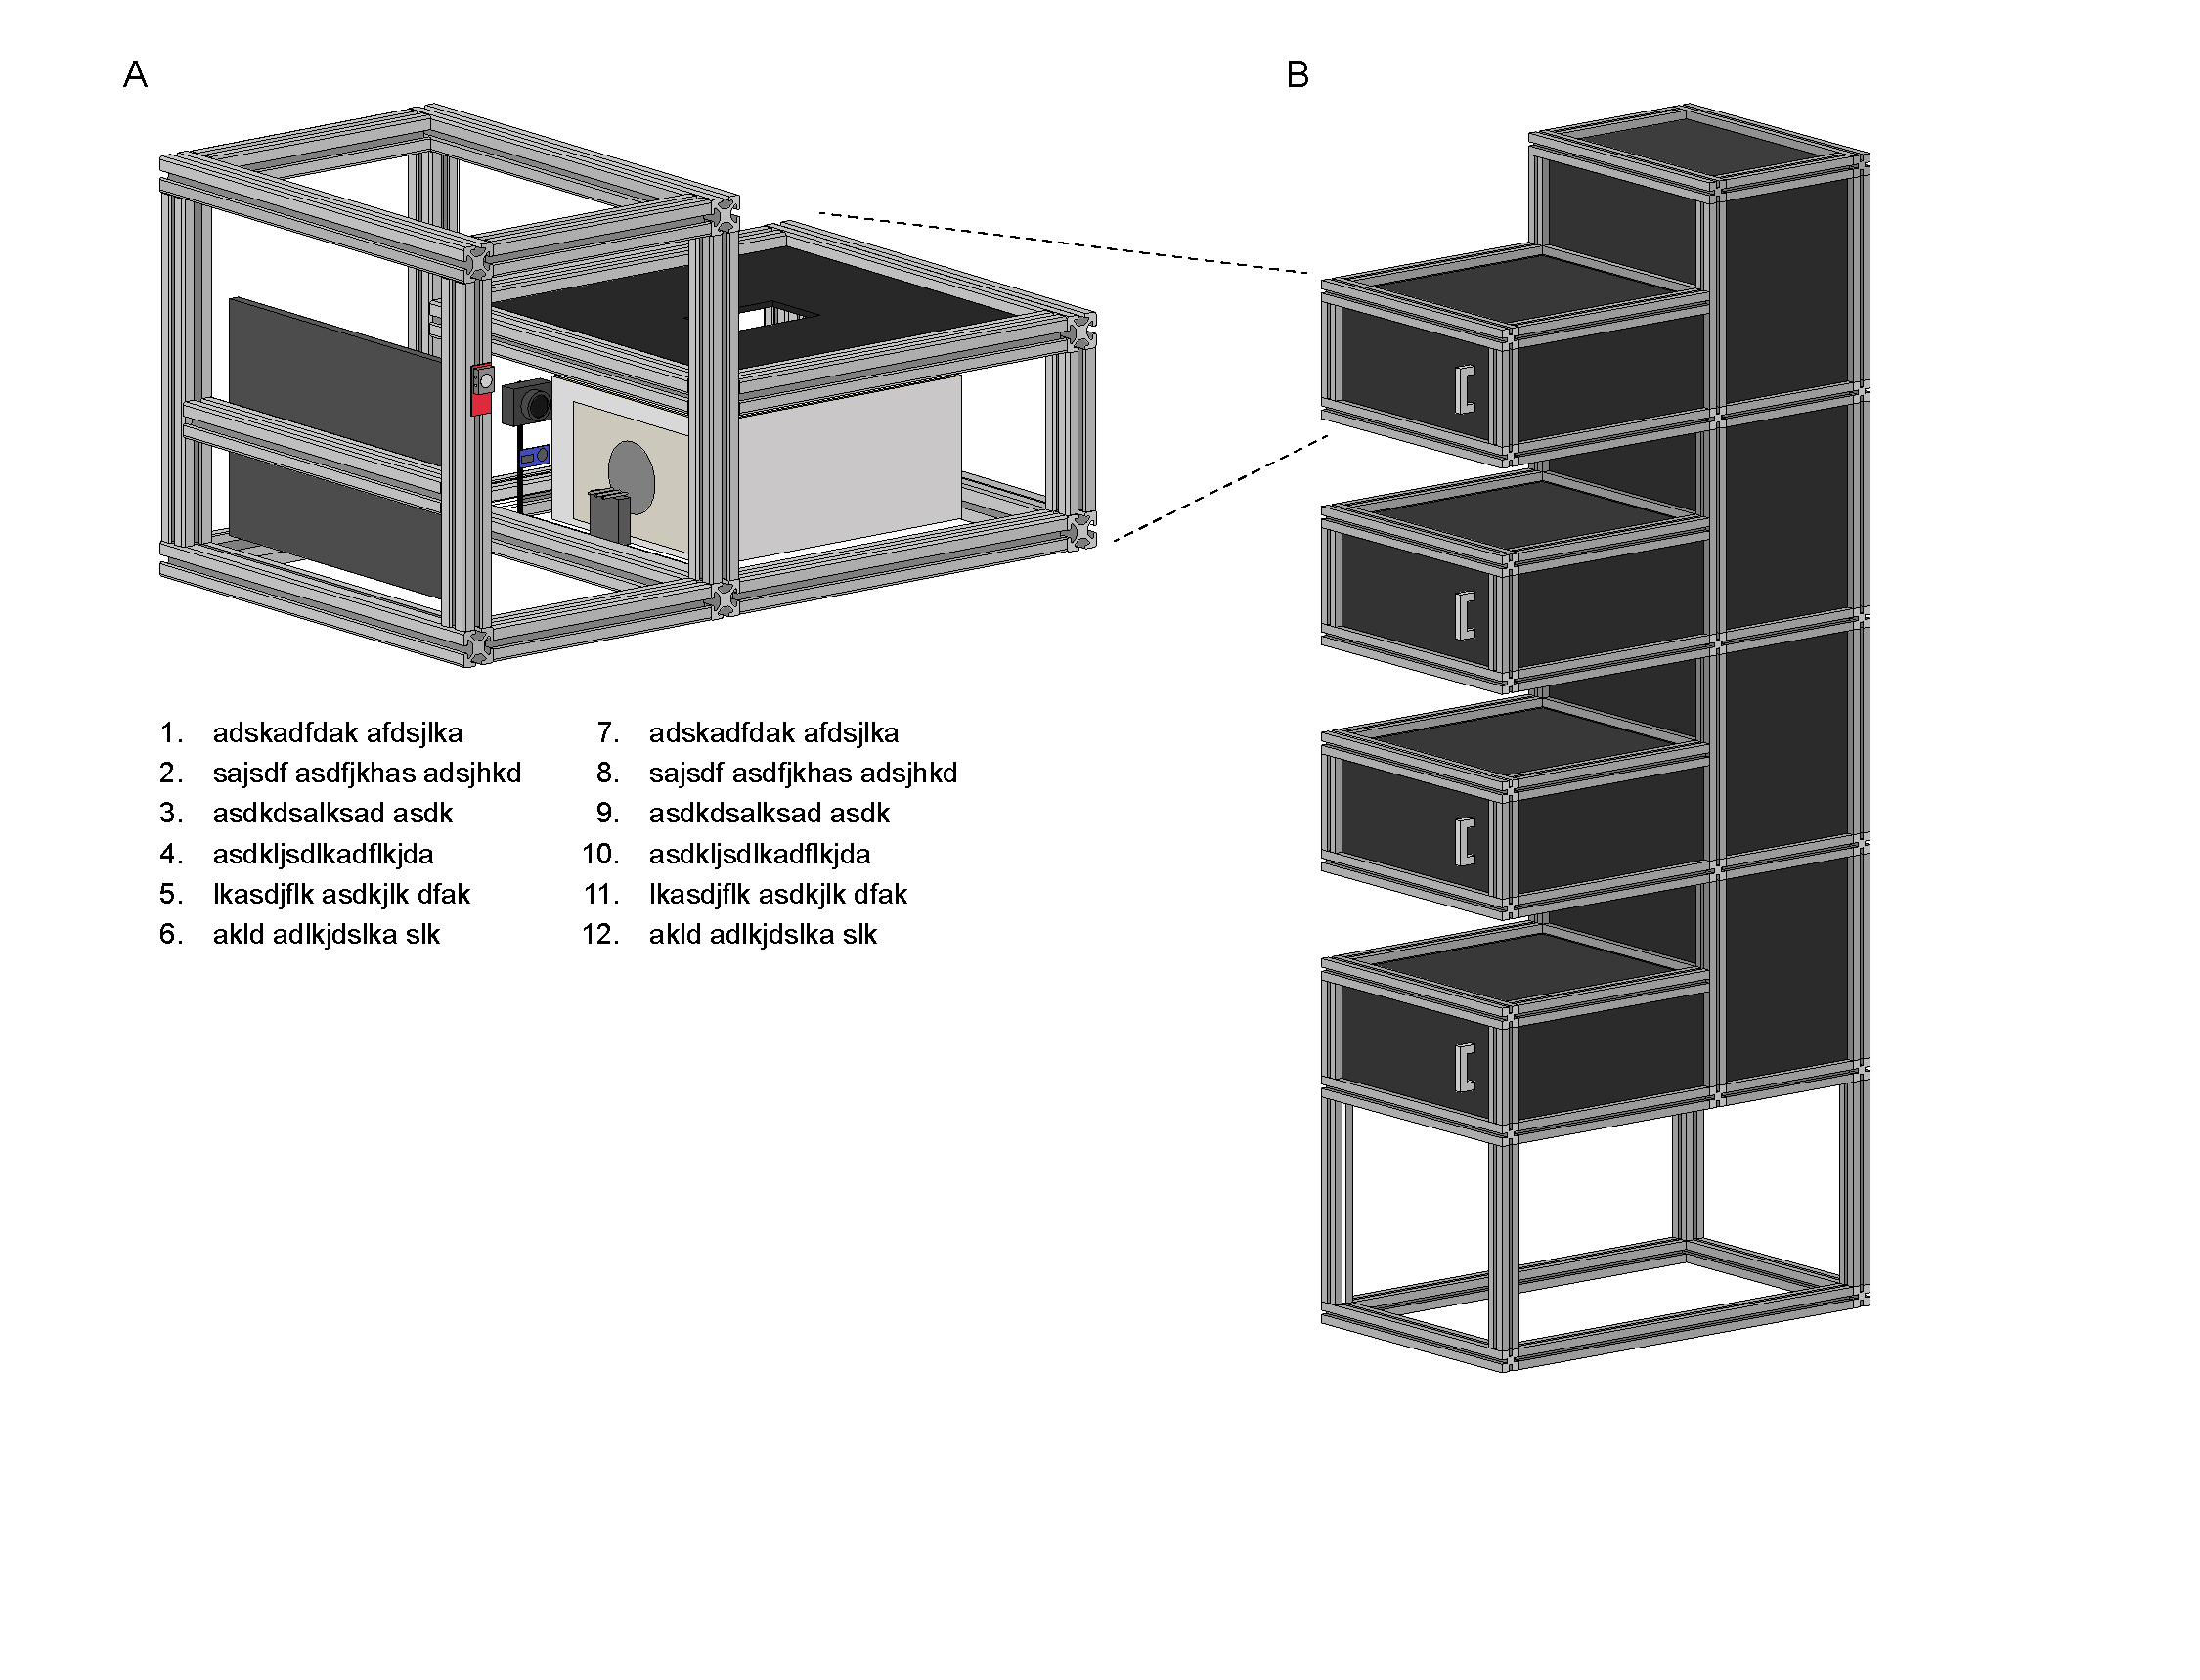
\includegraphics[width=\textwidth]{figures/chapter_1/ratbox_schematic.pdf}
    \vspace{.1in}
    \caption[OpenRatBox]{Schematic of OpenRatBox. \textbf{A.} One training box. Parts: 1. Home cage, 2. Sensors and reward ports, 3. USB camera and IR detector, 4. Monitor, 5. Solenoid valves, 6. Tubing and wiring leads out of the vestibule, etc. \textbf{B.} A full tower assembly of four identical training boxes. 
    \label{fig:ratbox_schematic}}
\end{figure}


\section{High-throughput training}
% FIGURE 1.2 Basic 2-choice task, high throughput

We trained rats to perform a simple two-category object discrimination task. Animals had to lick one response port for object ``A'', and another response port for object ``B''.  Animals could be trained to perform basic shape discriminations for reasonably dissimilar objects (\textit{e.g.} the objects in FIGUREXREFREF) in one month or less, and animals readily performed several hundred trials per day in the automated training rig. 


% FIGURE 1.2 Basic task acqusition
\begin{figure}[t!]
    \includegraphics[width=\textwidth]{figures/chapter_1/training_paradigm.pdf}
    \vspace{.1in}
    \caption[OpenRatBox]{Schematic of OpenRatBox. \textbf{A.} One training box. Parts: 1. Home cage, 2. Sensors and reward ports, 3. USB camera and IR detector, 4. Monitor, 5. Solenoid valves, 6. Tubing and wiring leads out of the vestibule, etc. \textbf{B.} A full tower assembly of four identical training boxes. 
    \label{fig:ratbox_schematic}}
\end{figure}


\section{Generating complex visual object stimuli}
Morph stimuli and stuff

% FIGURE 1.3 Stimulus generation

\section{Tests of visual object discrimination and recognition}
% FIGURE 1.3 INVARIANCE TEST

After learning the ``base'' object A/B task, animals were presented with two types of generalization tests. In the first, INVARIANT OBJE RECT.

% FIGURE 1.4 MORPHS
In the second test, samples from a morph line between the previously trained ``poles'' of the stimulus continuum. REFREF shows two-dimensional stimuli generated using closed non-uniform rational B-spline curves interpolating smoothly in the space of their control vertices. 

During the ``probe'' phase of the task, morphed samples were randomly interleaved roughly 10\% of the time, without feedback, during the ordinary discrimination task. These probe trials were then used to build up a psychophysical curve to determine the animals' naive behavior in classifying the objects as ``A'' or ``B''. 

These curves characterize the category boundary along the morph axis 


\begin{figure}
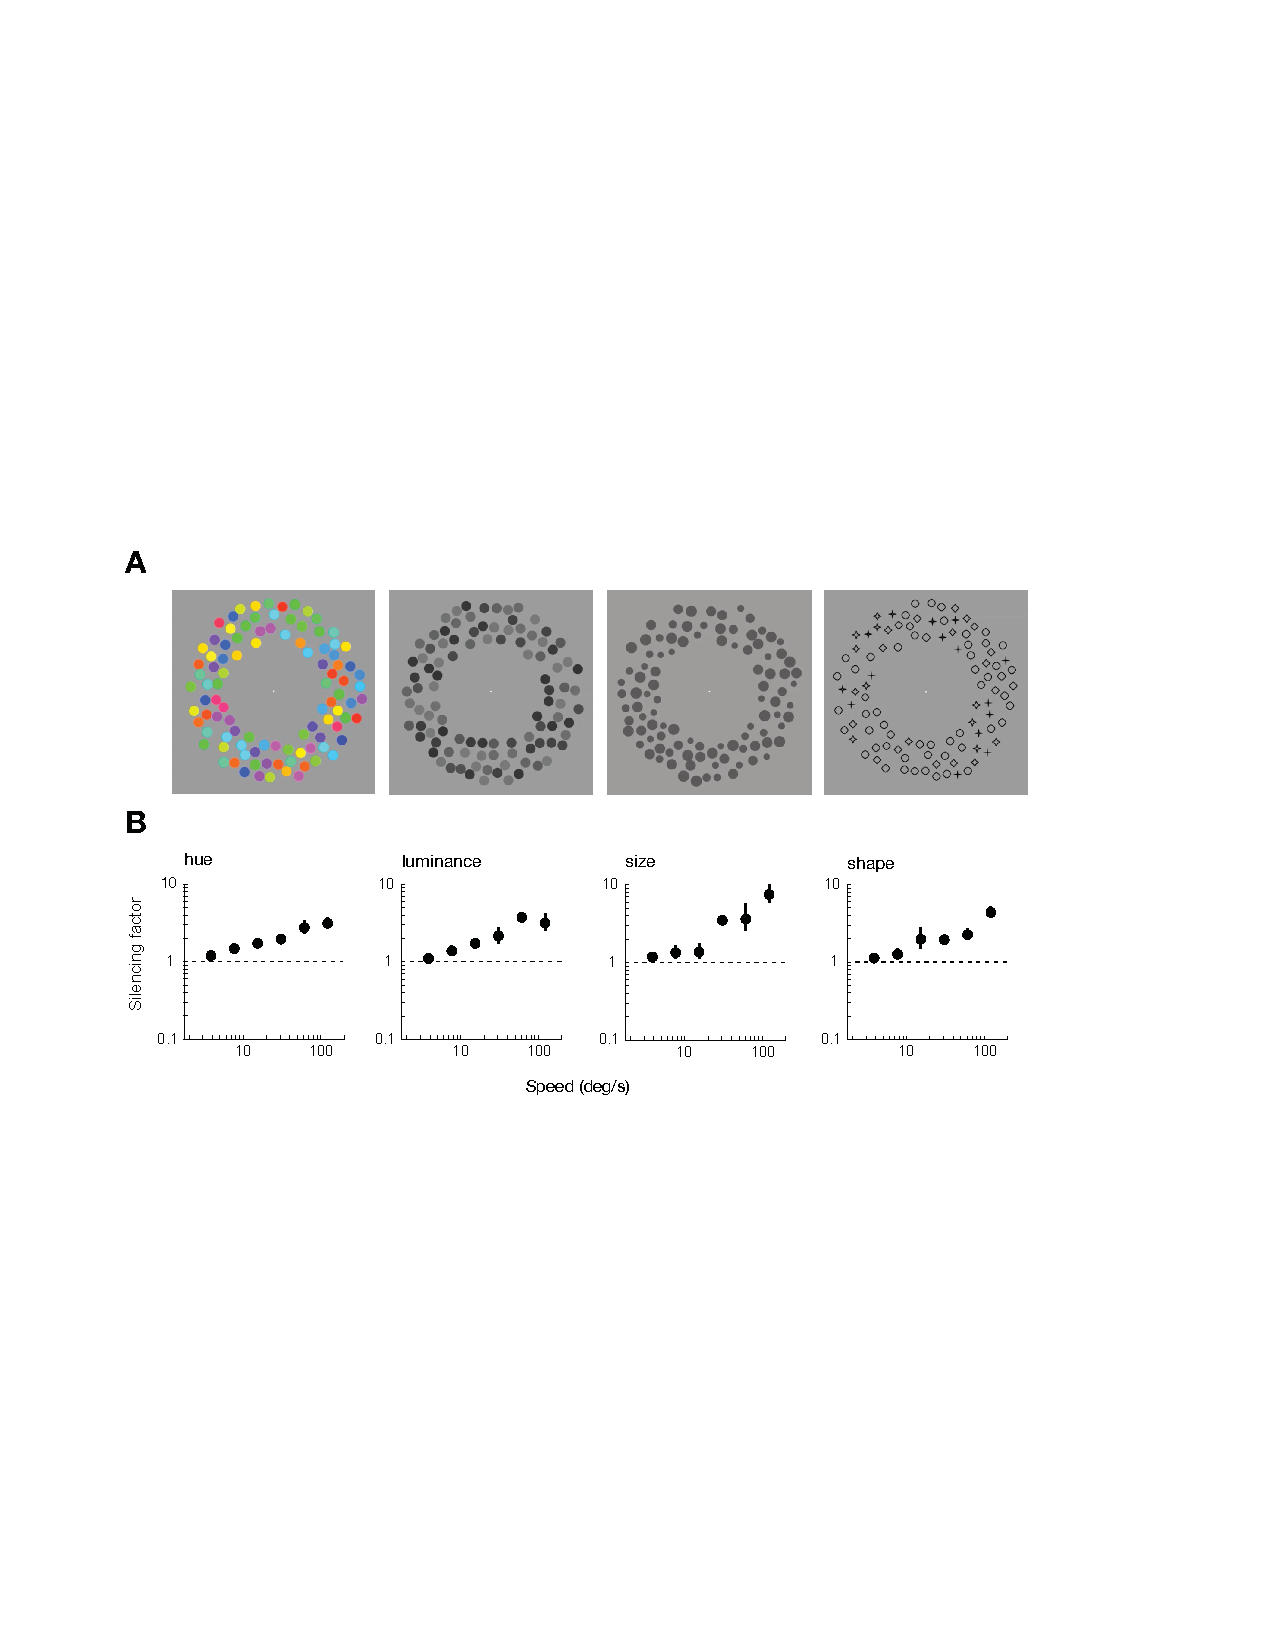
\includegraphics[width=\textwidth]{figures/fig1}
\caption[Short figure name.]{This is a figure that floats inline and here is its caption.
\label{fig:myInlineFigure}}
\end{figure}

Stuff can be written here



% \texttt{This is a line of code.}


% For an example of a full page figure, see Fig.~\ref{fig:myFullPageFigure}.

% % EXAMPLE FIGURE 
% \begin{figure}[t!]
%     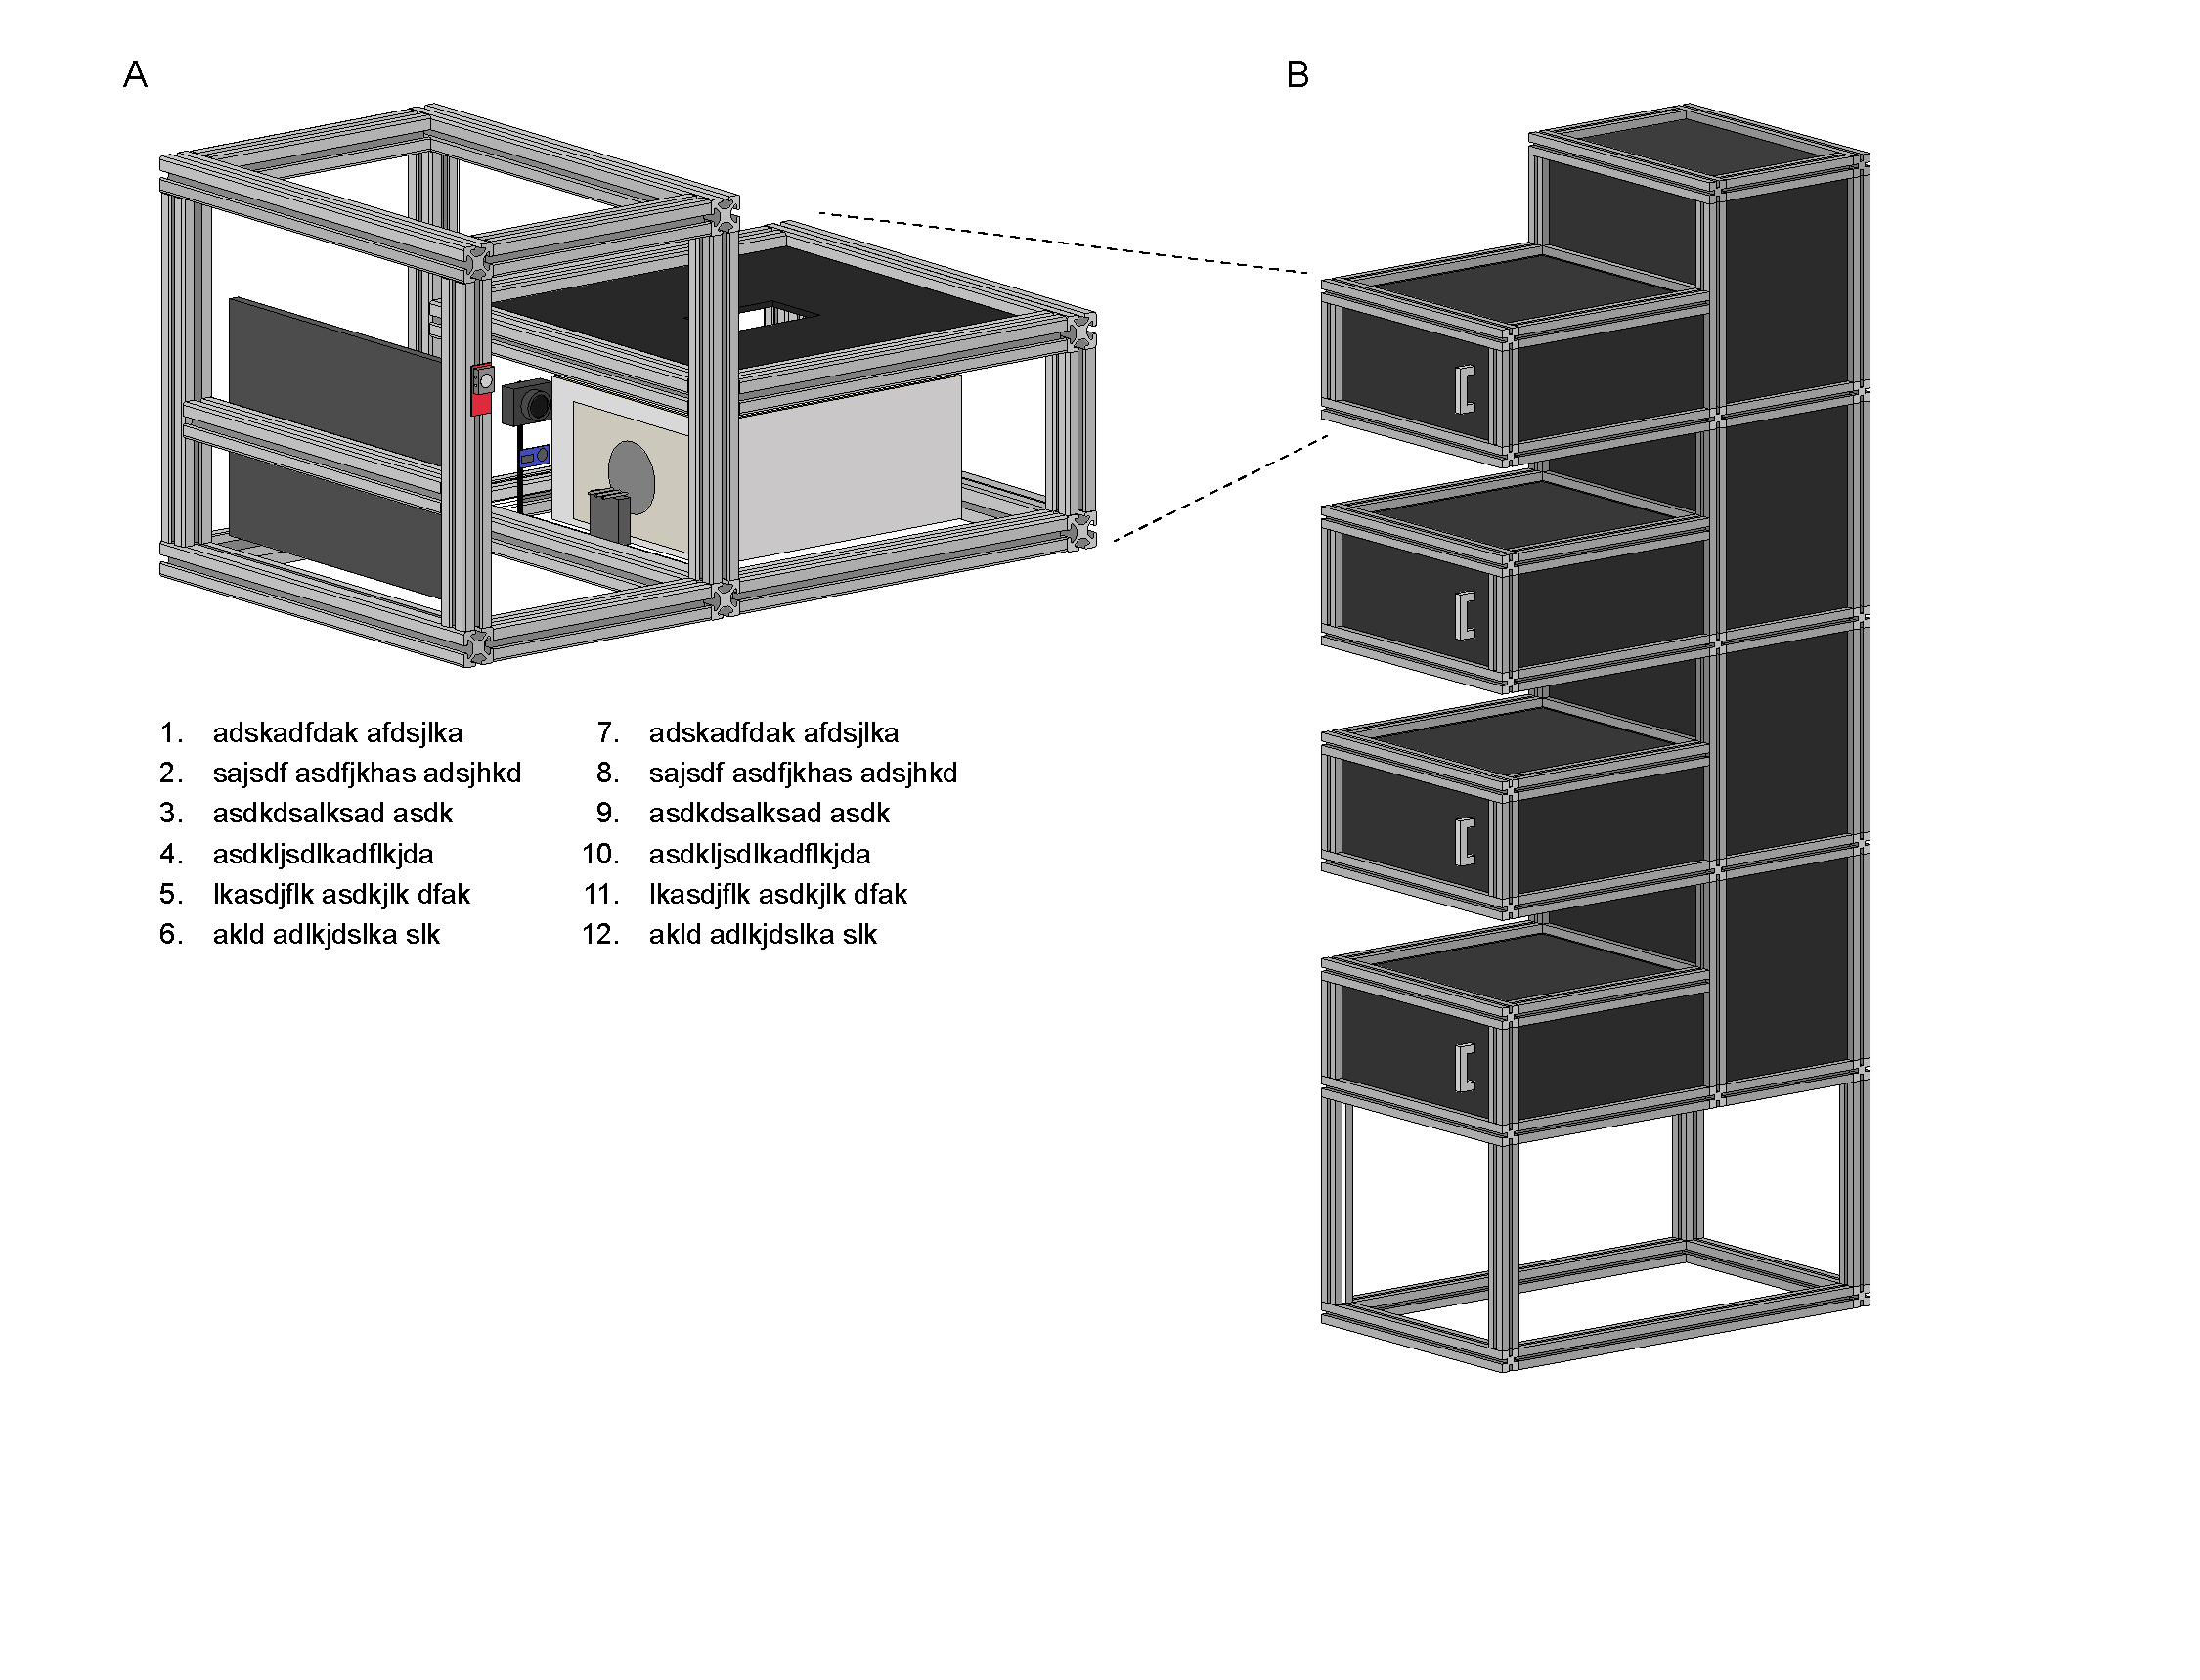
\includegraphics[width=\textwidth]{figures/chapter_1/ratbox_schematic.pdf}
%     \vspace{.1in}
%     \caption*{\textbf{Figure 2.1} Example figure and tips -- A) Your figure numbers should follow the format of Figure chapter#.figure#. B) Set width equal to textwidth. C) Specify position as [t!] to insert at page top.}
% \end{figure}

%% Requires fltpage2 package
%%
% \begin{FPfigure}
% 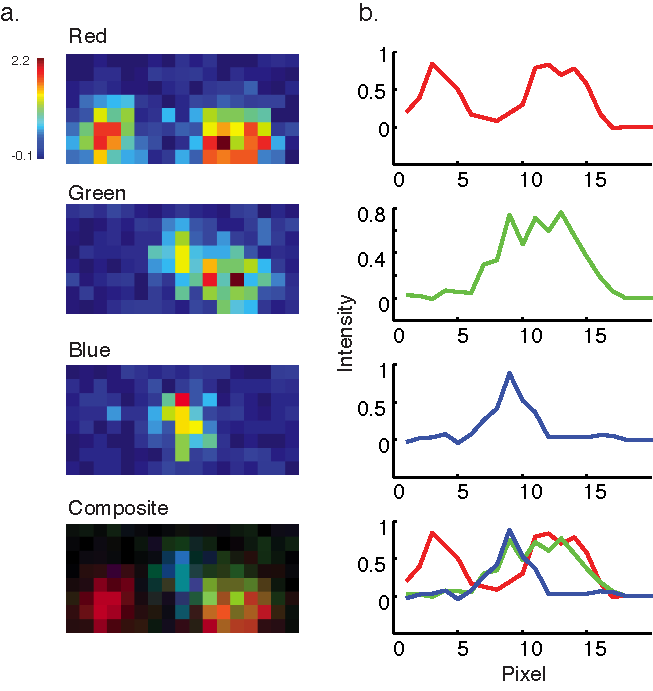
\includegraphics[width=\textwidth]{figures/fullpage}
% \caption[Short figure name.]{This is a full page figure using the FPfigure command. It takes up the whole page and the caption appears on the preceding page. Its useful for large figures. Harvard's rules about full page figures are tricky, but you don't have to worry about it because we took care of it for you. For example, the full figure is supposed to have a title in the same style as the caption but without the actual caption. The caption is supposed to appear alone on the preceding page with no other text. You do't have to worry about any of that. We have modified the fltpage package to make it work. This is a lengthy caption and it clearly would not fit on the same page as the figure. Note that you should only use the FPfigure command in instances where the figure really is too large. If the figure is small enough to fit by the caption than it does not produce the desired effect. Good luck with your thesis. I have to keep writing this to make the caption really long. LaTex is a lot of fun. You will enjoy working with it. Good luck on your post doctoral life! I am looking forward to mine. \label{fig:myFullPageFigure}}
% \end{FPfigure}
% \afterpage{\clearpage}

